%\documentclass{article}
\documentclass{tufte-handout}

%\geometry{showframe}% for debugging purposes -- displays the margins
\usepackage{pdfpages}
\usepackage{amsmath}
\usepackage{natbib}
\usepackage{booktabs}
\usepackage{multicol}
\usepackage[version=4]{mhchem} 

\bibfont{\small} % Doesn't see to work...
\usepackage{graphicx}

\setkeys{Gin}{width=\linewidth,totalheight=\textheight,keepaspectratio}
% \graphicspath{{graphics/}}

\newenvironment{itemize*}%
  {\begin{itemize}%
    \setlength{\itemsep}{0pt}%
    \setlength{\parskip}{0pt}}%
  {\end{itemize}}
	
\newenvironment{enumerate*}%
  {\begin{enumerate}%
    \setlength{\itemsep}{0pt}%
    \setlength{\parskip}{0pt}}%
  {\end{enumerate}}
	

\title{Particle Size Analysis of Soils by Sedimentation %\thanks{Isaac Medina}
}
\author[Marc Los Huertos]{Marc Los Huertos}
%\date{}  % if the \date{} command is left out, the current date will be used

% \SweaveOpts{prefix.string=graphics/plot} % Created a "graphics" subdirectory to 

\setsidenotefont{\color{blue}}

\usepackage{Sweave}
\begin{document}
\Sconcordance{concordance:Particle_Size_Analysis.tex:Particle_Size_Analysis.Rnw:%
1 39 1 1 0 11 1 1 5 39 1 1 3 1 2 230 1 1 7 10 1 1 8 4 1 1 9 18 0 1 2 21 1 1 4 4 0 1 6 3 0 %
1 2 6 1 1 10 1 2 19 1 1 10 1 1 1 7 1 2 244 1 1 4 2 1 1 5 7 0 1 2 4 1 1 2 7 0 1 2 4 1 1 14 %
16 0 1 2 6 1 1 2 14 0 1 2 45 1 1 4 6 0 1 2 88 1 1 2 1 0 2 1 1 2 1 0 1 3 1 0 2 1 2 2 4 1 2 %
2 12 0 1 5 4 1 1 2 1 0 1 2 5 0 1 1 3 0 1 2 69 1 4 0 1 3 3 1 4 0 1 3 3 1 4 0 1 3 7 1 4 0 1 %
3 2 1 1 3 2 0 4 1 1 4 5 0 1 2 2 1 1 2 7 0 1 2 3 1 1 3 5 0 1 2 27 1}


\maketitle% this prints the handout title, author, and date
\begin{abstract}
\noindent Soil is usually composed of particles with a mix of sizes where the relative proportion of size classes define the soil texture. As a property of a soil, the texture can determine water relations, bio-availability of nutrients and toxics, and soil biogeochemistry. Soil texture can be determined using qualitative or quantitative methods that might be employed in the field or in the laboratory, respectively. While classes are distinguished in the field and the class is then used to determine crop suitability and to approximate the soils responses to environmental and management conditions such as drought, fertility, or calcium (lime) requirements.
\end{abstract}

%\printclassoptions

% Setting up the margins, etc for R

\section{Outline and Outcomes}
This handout describes how soil samples can be quantitatively analyzed using hydrometer to promote the following skills:

\begin{enumerate}
	\item Understand the equations that describe how particle size and the terminal velocity in a suspension;
	\item Use sedimentation methods to measure density changes in soil suspensions; and
	\item Apply equations to calculate the density and percent of a sample in suspension to calculate the particle sizes of a soil sample. 
\end{enumerate}

\section{Background}

Soils are composed of mineral particles, organic matter, water and air. In general, most of the mass of soil is composed of mineral particles and the size or texture of these particles influence a range of physical and biological processes in soil. In the simplest cases, we can categorize the size of particles into three groups: Sand, silt, and clay. In general, we consider soil to be made up of particles that can pass through a 2 mm sieve, aka No. 10 sieve (Figure \ref{fig:8stainless_sieve}). 

\begin{marginfigure}
	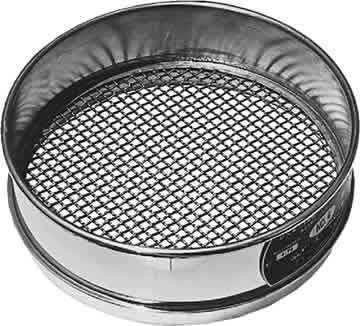
\includegraphics{8stainless_sieve.jpg}
	\caption{Sieves are circular dishes with a mesh bottom. Each sieve type have different mesh sizes, thus can be used to ``split'' soils based on the size of particles, where particles smaller than the mesh fall through and larger particles are retained.}
	\label{fig:8stainless_sieve}
\end{marginfigure}

\begin{table}
		\begin{tabular}{lrr}\hline
Classification 					&  USDA System 		& World Reference Base\\ \hline\hline
			Clay 							& <0.002 mm 			& <0.002 mm \\
			Silt 							& 0.002-0.05 mm 	& 0.002-0.063 mm\\
			Very fine sand		& 0.05-0.10 mm 		& 0.063-0.0125 mm\\
			Fine sand 				& 0.10-0.25 mm 		& 0.0125-0.20 mm\\
			Medium sand				& 0.25-0.50 mm 		& 0.20-0.63 mm\\
			Coarse sand 			& 0.50-1.00 mm 		& 0.63-1.25 mm\\
			Very coarse sand	& 1.00-2.00 mm 		& 1.25-2.00 mm\\
			Gravel 						& >2.0 mm 				& >2.0 mm \\ \hline
		\end{tabular}
\end{table}


There are a number of references that explain various methods to conduct a particle analysis, such as \citep{gee1986particle, day1965particle, beretta2014soil}. For our purpose, we will use the method developed by the ASTM International that capitalizes on the correlation between the size of particles, their terminal velocity, and the density of the suspension \citep{standard2007d422}. 

This handout describes how we can use a hydrometer to measure density of a soil suspension and how this density changes with time. As the density changes, we can use several equations to estimate the proportion of particle sizes. 

\begin{figure}
